% --- Inserir folha de aprovação --- %

% Isto é um exemplo de Folha de aprovação, elemento obrigatório da NBR
% 14724/2011 (seção 4.2.1.3). Você pode utilizar este modelo até a aprovação
% do trabalho. Após isso, substitua todo o conteúdo deste arquivo por uma
% imagem da página assinada pela banca com o comando abaixo:

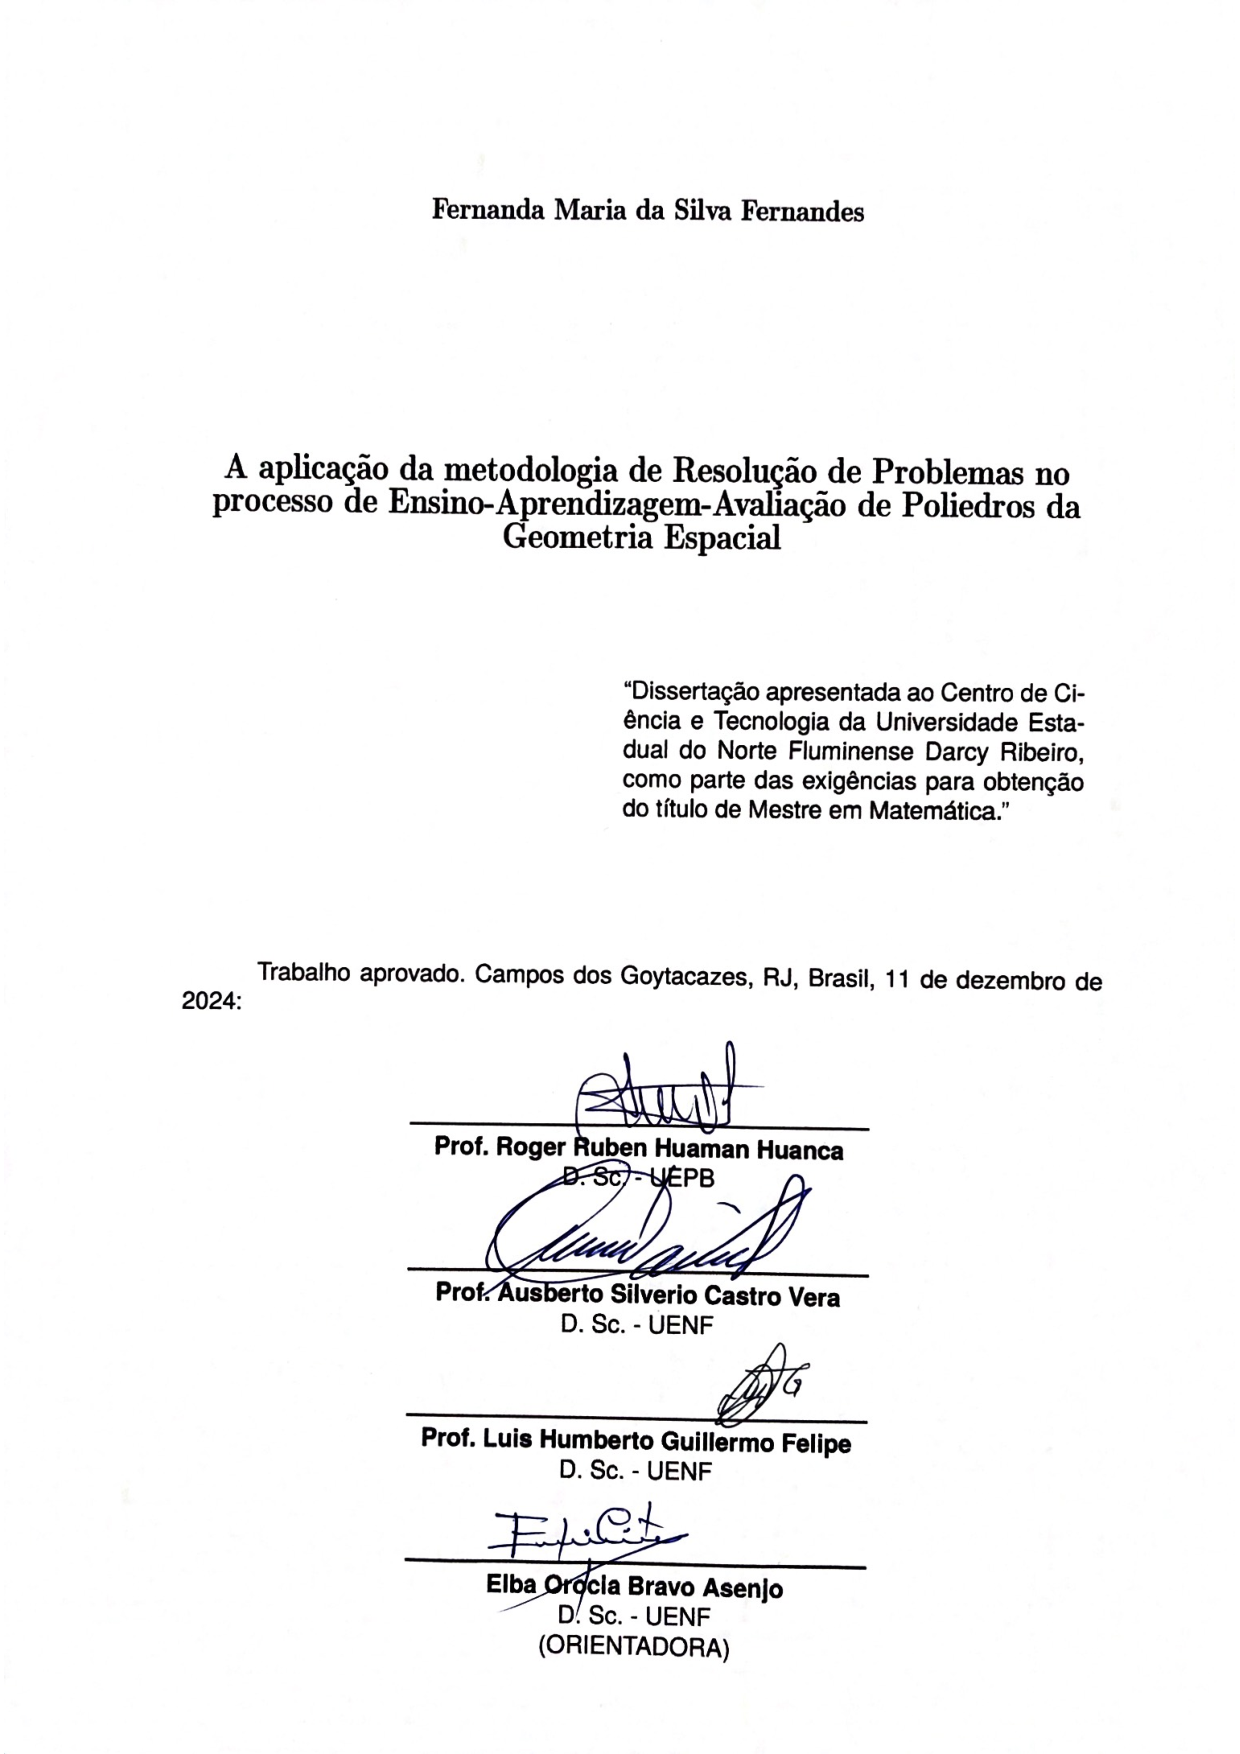
\includepdf{PDFs/FolhaDeAprovação.pdf}

\begin{comment}

\begin{folhadeaprovacao}

  \begin{center}
    {\ABNTEXchapterfont\large\imprimirautor}

    \vspace*{\fill}\vspace*{\fill}
    {\ABNTEXchapterfont\bfseries\Large\imprimirtitulo}
    \vspace*{\fill}

    \hspace{.45\textwidth}
    \begin{minipage}{.5\textwidth}
      \imprimirpreambulo
    \end{minipage}%
    \vspace*{\fill}
  \end{center}

  Trabalho aprovado. Campos dos Goytacazes, RJ, Brasil, 11 de dezembro de 2024:

  \assinatura{\textbf{Prof. Roger Ruben Huaman Huanca}\\ D. Sc. - UEPB}
  \assinatura{\textbf{Prof. Ausberto Silverio Castro Vera}\\ D. Sc. - UENF}
  \assinatura{\textbf{Prof. Luis Humberto Guillermo Felipe}\\ D. Sc. - UENF}
  \assinatura{\textbf{Elba Orocia Bravo Asenjo} \\ D. Sc. - UENF\\ (ORIENTADORA)}

  % \begin{center}
  %   \vspace*{0.5cm}
  %   {\large\imprimirlocal}
  %   \par
  %   {\large\imprimirdata}
  %   \vspace*{1cm}
  % \end{center}

\end{folhadeaprovacao}
\end{comment}
